% Setup - do not change
\documentclass[11pt]{article}
\usepackage[top=0.9in, left=0.9in, bottom=0.9in, right=0.9in]{geometry} 
\usepackage{parskip}
\usepackage{float}
\usepackage[english]{babel}
\usepackage[utf8]{inputenc}
\usepackage{amsmath,amsthm,amssymb,graphicx,pdfpages,lipsum,hyperref}
\usepackage[none]{hyphenat}
\usepackage{csquotes}
\usepackage{wrapfig}
% \usepackage{multirow}
% \usepackage{booktabs}

\setlength\parindent{0pt}
%%%%%%%%%%%%%%%%%%%%%%%%%%%%%%%%%%%%%%%%%%%%%%%%%%%%%%%%%%%%%%%%%%%
% add other packages here if required

%% Bibliography are specified in this file. You can also choose inline bib style if you want to. But make sure your citation style is consistent (and proper)
% For more details on citation: https://library.unimelb.edu.au/recite
\usepackage[sorting = none]{biblatex}
\addbibresource{references.bib}

%%%%%%%%%%%%%%%%%%%%%%%%%%%%%%%%%%%%%%%%%%%%%%%%%%%%%%%%%%%%%%%%%%% the '%' symbol denotes comments

% Begin document creation
% DELETE THE \lipsum PLACEHOLDERS WHEN YOU BEGIN
\title{\textbf{Explore the factors that affect drivers' income per order during the COVID-19}}
\author{
Jingxi Yuan \\
Student ID: 1213860 \\
%% Replace the link with your github repo
% 1. Remember to escape underscore (\_) in the link.
% 2. Remember to include the commit you want to submit in the link
\href{https://github.com/MAST30034-Applied-Data-Science/mast30034\_p1\_template/tree/fd9f1dd17fdbcb5b119b70c93a22da8210d44fd7}{Github repo with commit}
}

\begin{document}

\maketitle

\section{Introduction}
Because taxi drivers in New York City receive thousands of orders every day. In order to facilitate management and statistics, the New York government has recorded annual yellow and green taxi and rental vehicle ("FHV") trip records on The New York City Taxi and Limousine Commission (TLC) since 2009. Due to the COVID-19 outbreak, New York City's economy has been impacted like never before. Newly released city data shows that the coronavirus pandemic has devastated New York City's taxi workforce (David, 2020)\cite{1}. This report hopes to analyze the variables that affect the revenue of New York taxi drivers per order during COVID-19 through data released by TLC and NYC Health.
This report will by plotting and comparing contour plots, look at which areas of New York City drivers received higher income per order during COVID-19. And compare the impact of variables in the trip records of yellow taxis on driver income by analyzing data and building a linear model and using the linear model and mutual information to determine the impact of the epidemic on driver income.
\subsection{Data}
This data selects the yellow taxi data and Covid-19 case data from 12/2021 to 02/2022.
\subsubsection {yellow taxi data\cite{3}}
The reason for choosing yellow taxis as the data for this report research is that only yellow taxis can pick up passengers in any area of New York City, reducing the impact of judging driver income due to the type of taxi that cannot pick up passengers in some areas. The data selected for this report include:
\begin{itemize}
    \item "tpep\_pickup\_datetime" and 'tpep\_dropoff\_datetime'. Pick-up time and drop-off time can calculate the total time the driver spends on a single order.
\end{itemize}
\begin{itemize}
    \item "trip\_distance". Travel distance helps exclude unreasonable data. For example, the trip distance is 1000 miles, but only 20 dollars is charged.
\end{itemize}
\begin{itemize}
    \item "PULocationID" and "DOLocationID". The location id of getting on and the location id of getting off can help draw a map.
\end{itemize}
\begin{itemize}
    \item "payment\_type", "fare\_amount" and "tip\_amount". Payment method, far amount, and tip amount are used to analyze the driver's revenue per order.
\end{itemize}
This report assumes that the driver's income is only far\_amount and tip\_amount, and the calculation method of far\_amount is 2.5 * trip\_distance + 2.5.\cite{4}
\subsubsection {COVID-19}
Regarding covid-19, this report selects the data provided by NYC Health on the number of total COVID-19 cases occurring each day and the number of covid-19 cases by region\cite{2}. As shown in Figure 1, the peak period of COVID-19 is from 12/2021 to 01/2022. This data can display the number of cases that occurred every day from 12/2021 to 02/2022, which is convenient for comparison with the yellow taxi data. Compare and build models. Among them, 12/2021 to 01/2022 is the number of covid cases during the epidemic, 02/2022 is the number of covid cases after the epidemic, and 02/2022 is used as the control group. The data-by-day data includes:
\begin{itemize}
    \item Date and the total number of cases. The date and the total number of cases were used to identify the month used for this report and were used to build a model along with driver earnings to analyze whether COVID-19 had an impact on driver earnings.
\end{itemize}
\begin{itemize}
    \item The number of cases in each region. The number of cases by region is used to help analyze the map.
\end{itemize}
\begin{wrapfigure}{r}{7cm}
    \centering
    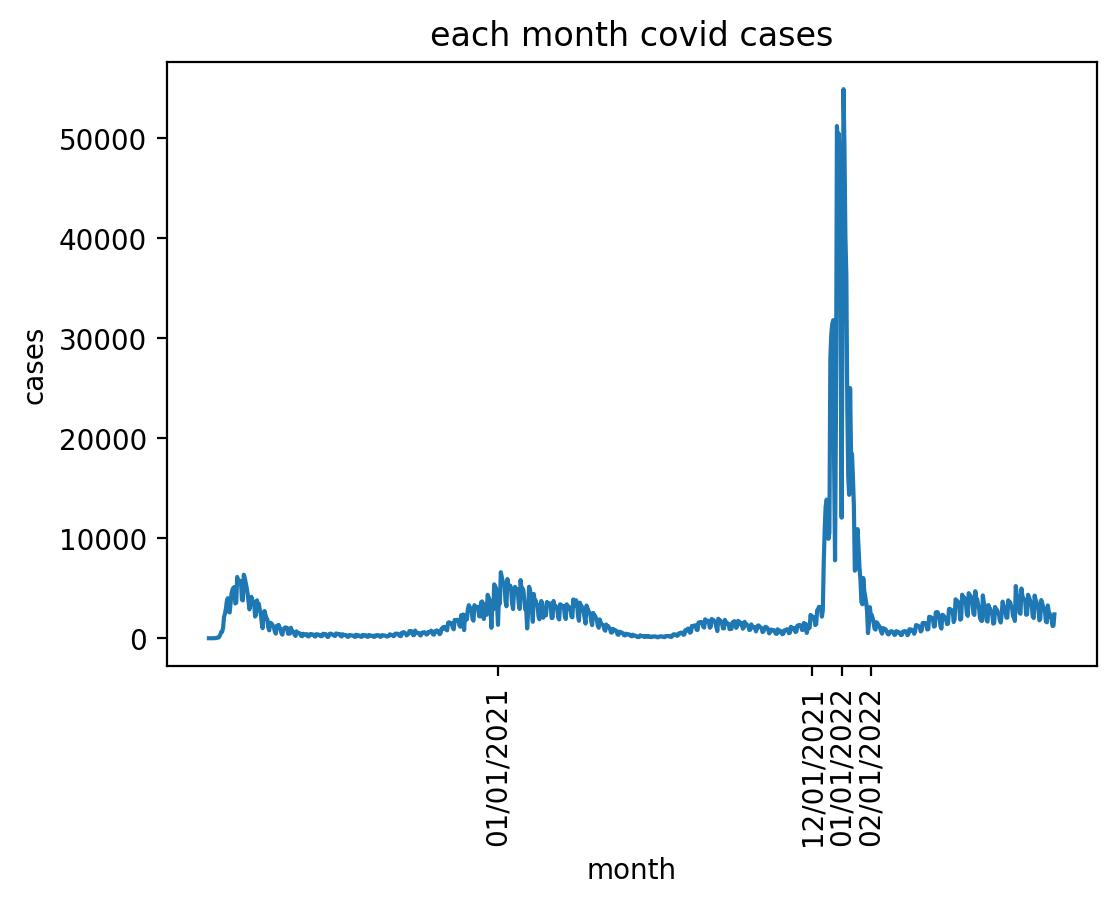
\includegraphics[width=0.5\textwidth]{plots/each month covid cases}
    \caption{}
    \label{fig:my_label}
\end{wrapfigure}
\subsection{new\_zones}
Finally merged shp and zones together to create new\_zones to help map New York City. The columns of new\_zones used in this report are:
\begin{itemize}
    \item LocationID: Confirm the map location
\end{itemize}
\begin{itemize}
    \item Geometry: Confirm latitude and longitude
\end{itemize}
\section{Processing the data}
\subsection{cleaning data}
Due to the yellow taxi data, there will be some unreasonable data, for example, the trip\_distance is hundreds of thousands of miles, but the driver only receives 10 dollars. Covid-19 data also has redundant dates. Therefore, processing is required before analysis.
\subsubsection{yellow taxi data}
\begin{itemize}
    \item After checking that no null data appears
\end{itemize}
\begin{itemize}
    \item Delete the data whose pickup time is not between 2021-12-01 00:00:00 and 2022-02-28 23:59:59
\end{itemize}
\begin{figure}[H]
  \begin{minipage}[b]{0.5\textwidth} 
    \centering 
    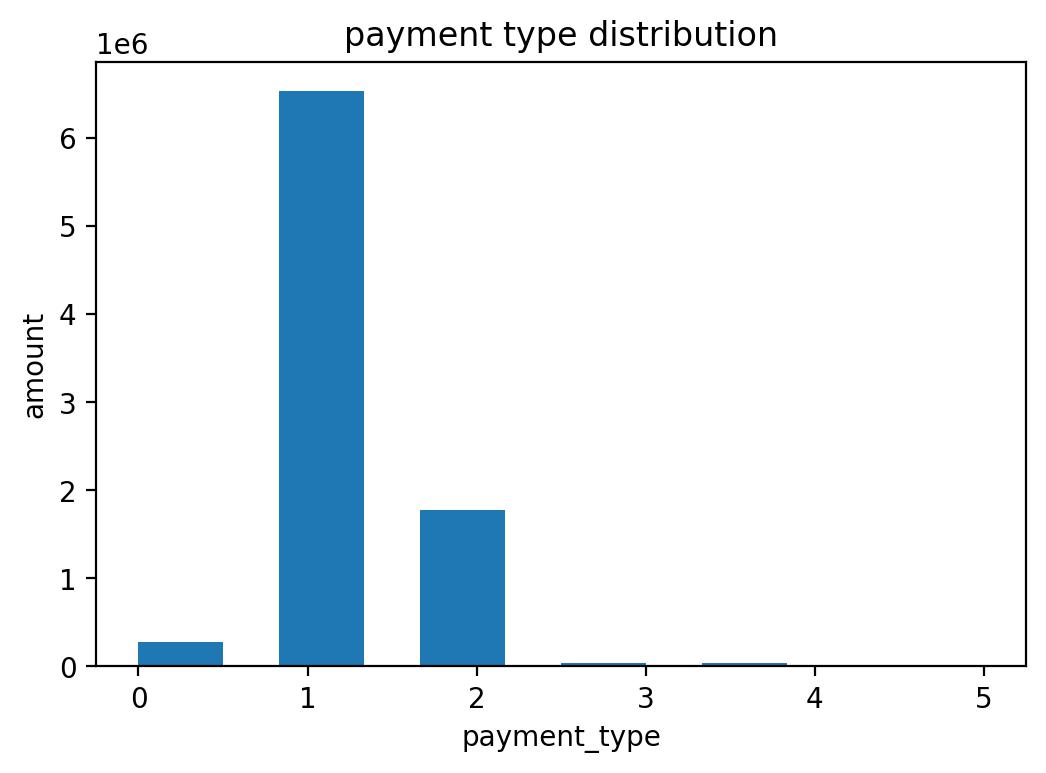
\includegraphics[width=0.9\textwidth]{plots/payment type distribution.jpg} 
    \caption{payment type}
    \label{fig:by:table} 
  \end{minipage}% 
  \begin{minipage}[b]{0.5\textwidth} 
    \centering
    \begin{tabular}{|c|c|c|} \hline 
      & fare\_amount & tip\_amount \\ \hline\hline 
      count & 8.580323e+06 & 8.580323e+06 \\
      mean &	1.357117e+01 &	2.524190e+00 \\
      std &	1.261778e+01 &	2.933317e+00 \\
      min &	-5.800000e+02 &	-9.801000e+01 \\
      25\% &	6.500000e+00 &	9.000000e-01 \\
      50\% &	9.500000e+00 &	2.060000e+00 \\
      75\% &	1.500000e+01 &	3.160000e+00 \\
      max &	3.009000e+03 &	8.888800e+02 \\
      \hline 
    \end{tabular} 
    \caption{}
    \label{tab:my_label}
\end{minipage} 
\end{figure}
\begin{figure}[H]
    \centering
    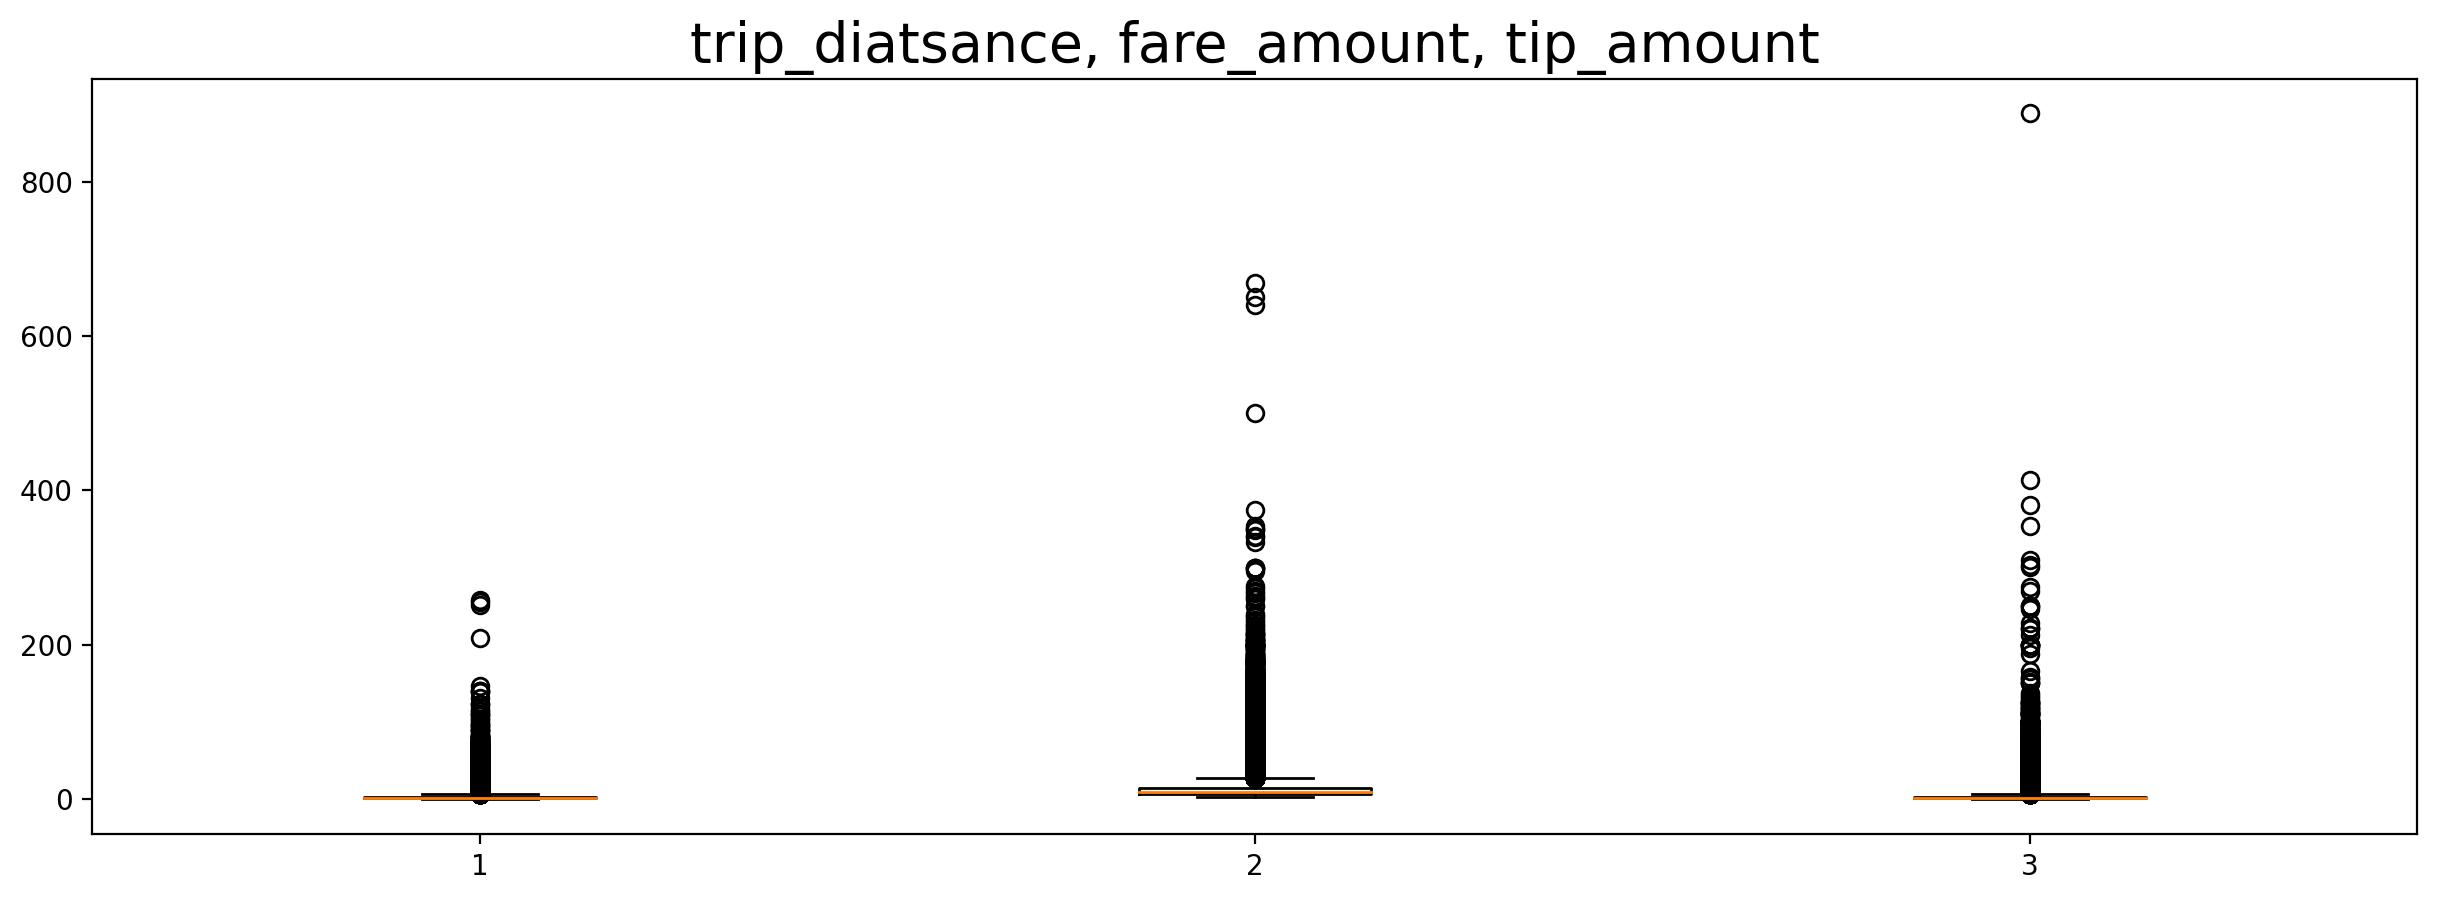
\includegraphics[width=0.7\textwidth]{plots/trip_diatsance, fare_amount, tip_amount.jpg}
    \caption{}
    \label{fig:my_label}
\end{figure}
\begin{itemize}
    \item As shown in Figure 2, since the number of payment methods 4, 5, and 6 is too small, they will be deleted without consideration.
\end{itemize}
\begin{itemize}
    \item As shown in Figure 3, both fare\_amount and tip\_amount have negative numbers, which is unreasonable. According to the New York taxi requirements, the initial charge is \$2.50. So fare\_amount should be greater than 2.5, tip\_amount should be greater than 0, and delete data smaller than them.
\end{itemize}
\begin{itemize}
    \item According to Figure 4, there are still many outliers, so delete the outliers.
\end{itemize}
\subsubsection{COVID-19 data}
\begin{itemize}
    \item Delete data not belonging to 12/01/2021 to 02/28/2022.
\end{itemize}
\subsection {Preprocessing}
\begin{itemize}
    \item Add a new variable - 'minutes' based on the yellow taxi data. Time = Drop off time - pick up time.
\end{itemize}
\begin{itemize}
    \item Since the cash tips are not included in the data, the original credit tips are used to estimate the cash tips, and then the fare amount and tip amount are added together to form a new variable – ‘income’.
\end{itemize}
\begin{itemize}
    \item As shown in Figure 5, minutes cannot be a negative number, so delete minutes less than 0.
\end{itemize}
\begin{figure}
  \begin{minipage}[b]{0.5\textwidth} 
    \centering
    \begin{tabular}{c|c|c} \hline
    & minutes & income\_rate \\ \hline
    count & 7.451040e+06 &	7.451040e+06 \\
    mean & 1.305993e+01 & inf \\
    std & 6.266184e+01 & NaN \\
    min & -1.044726e+05 & -1.632000e+03 \\
    25\% &	6.450000e+00 & 9.579399e-01 \\
    50\% &	1.008333e+01 &	1.113427e+00 \\
    75\% &	1.503333e+01 &	1.335977e+00 \\
    max & 2.933652e+04 & inf\\
    \hline
    \end{tabular} 
    \caption{}
    \label{tab:my_label}
  \end{minipage}% 
  \begin{minipage}[b]{0.5\textwidth} 
    \centering 
    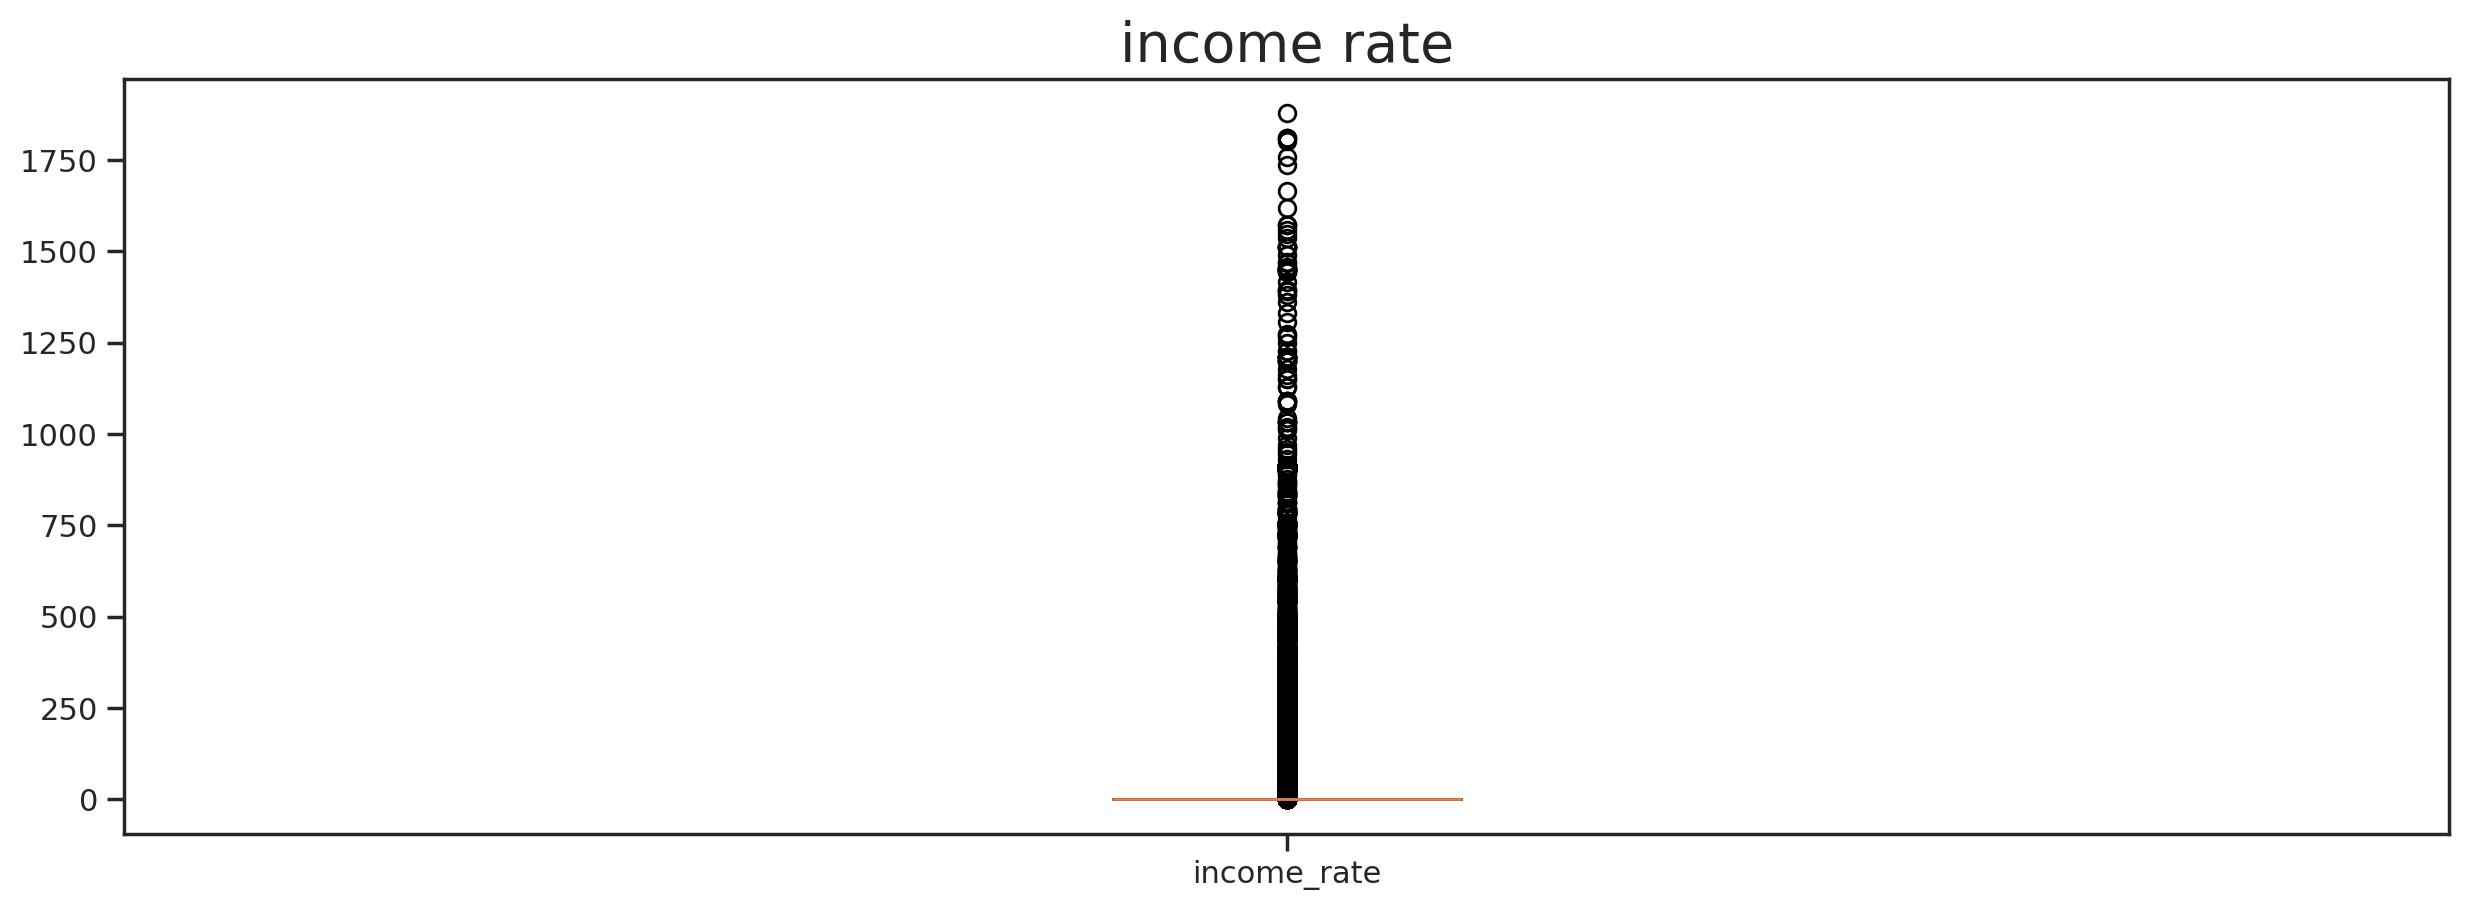
\includegraphics[width=0.9\textwidth]{plots/income rate.jpg} 
    \caption{payment type}
    \label{fig:by:table} 
\end{minipage} 
\end{figure}
\begin{itemize}
    \item As shown in Figure 6, outliers may affect the judgment of the model, so delete outliers.
\end{itemize}
\begin{itemize}
    \item To observe the impact of weekends and peaks, create two new variables – 'hour' and 'day'.
\end{itemize}
\section{Visualization}
\begin{itemize}
    \item According to Figure 7, it can be seen that during the epidemic, drivers generally make more money from 4:00 to 6:00 in the morning, and less from 8:00 to 15:00. This data looks strange. It may be because most of the people who call taxis from 3 to 6 are people who go home from entertainment activities at night. These people are richer and give more tips.
\end{itemize}
\begin{itemize}
    \item According to Figure 8, it can be seen that the driver earns more on weekends and the least on Thursdays. This picture looks a lot more reasonable, with more people coming out on weekends and Mondays. The reason for the low orders on Wednesday and Thursday is not clear, but it may be related to the national conditions of the United States.
\end{itemize}
\begin{itemize}
    \item The variables in Figure 9 are income rate, trip distance, PULocationID, fare amount, tip amount, minutes in order from top to bottom. The variables in Figure 10 are income\_rate, CASE\_COUNT,	BX\_CASE\_COUNT, BK\_CASE\_COUNT,	MN\_CASE\_COUNT,	QN\_CASE\_COUNT, SI\_CASE\_COUNT in order from top to bottom. 
\end{itemize}
\begin{figure}[H]
\centering
\begin{minipage}{.5\textwidth}
  \centering
  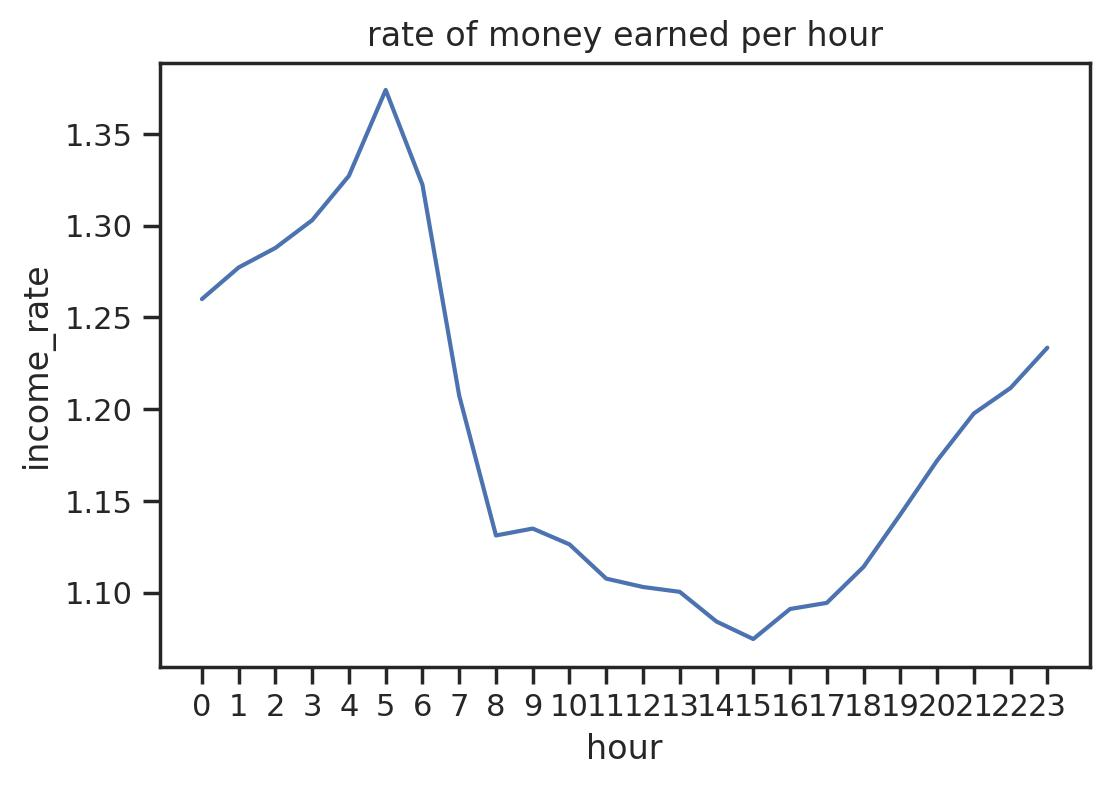
\includegraphics[scale=0.5]{plots/rate of money earned per hour.jpg}
  \caption{}
  \label{fig:by:table}
\end{minipage}%
\begin{minipage}{.5\textwidth}
  \centering
  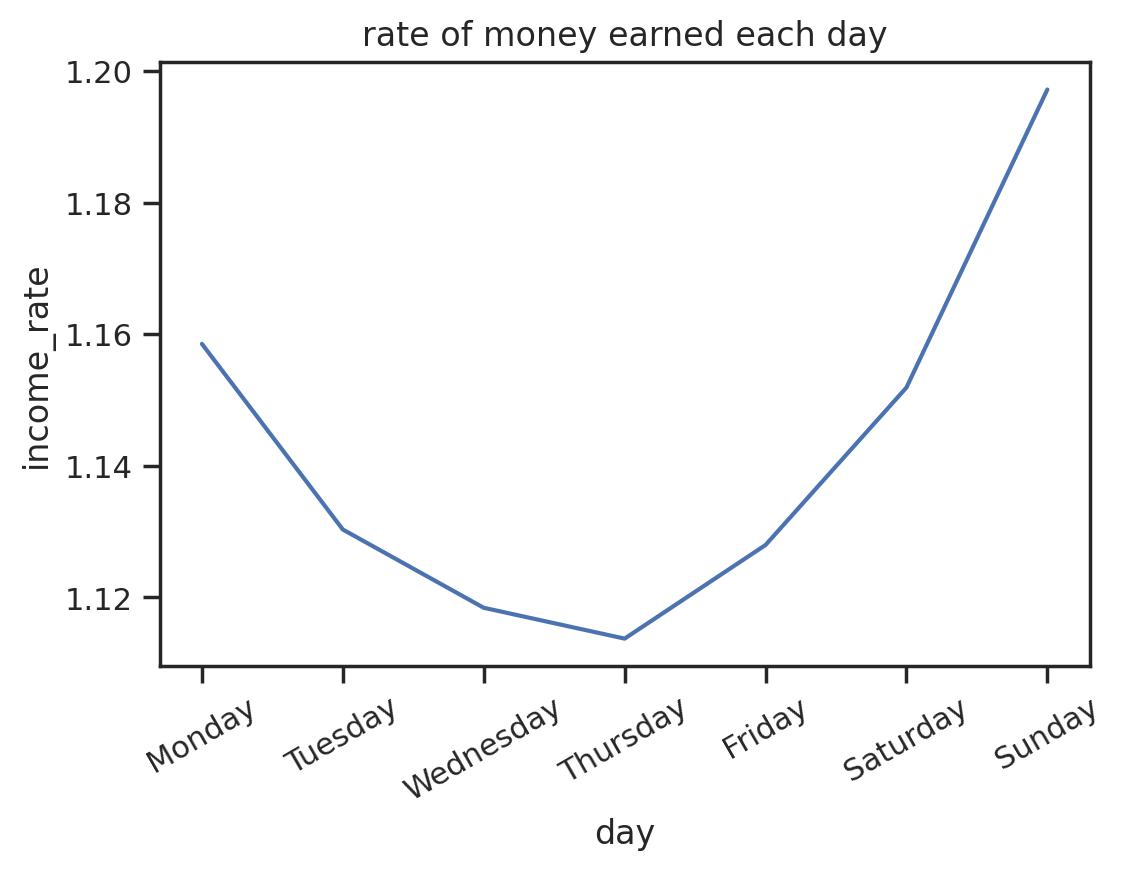
\includegraphics[width=.8\textwidth]{plots/rate of money earned each day.jpg}
  \caption{}
  \label{fig:by:table}
\end{minipage}
\end{figure}
\begin{figure}[H]
\centering
\begin{minipage}{0.4\textwidth}
  \centering
  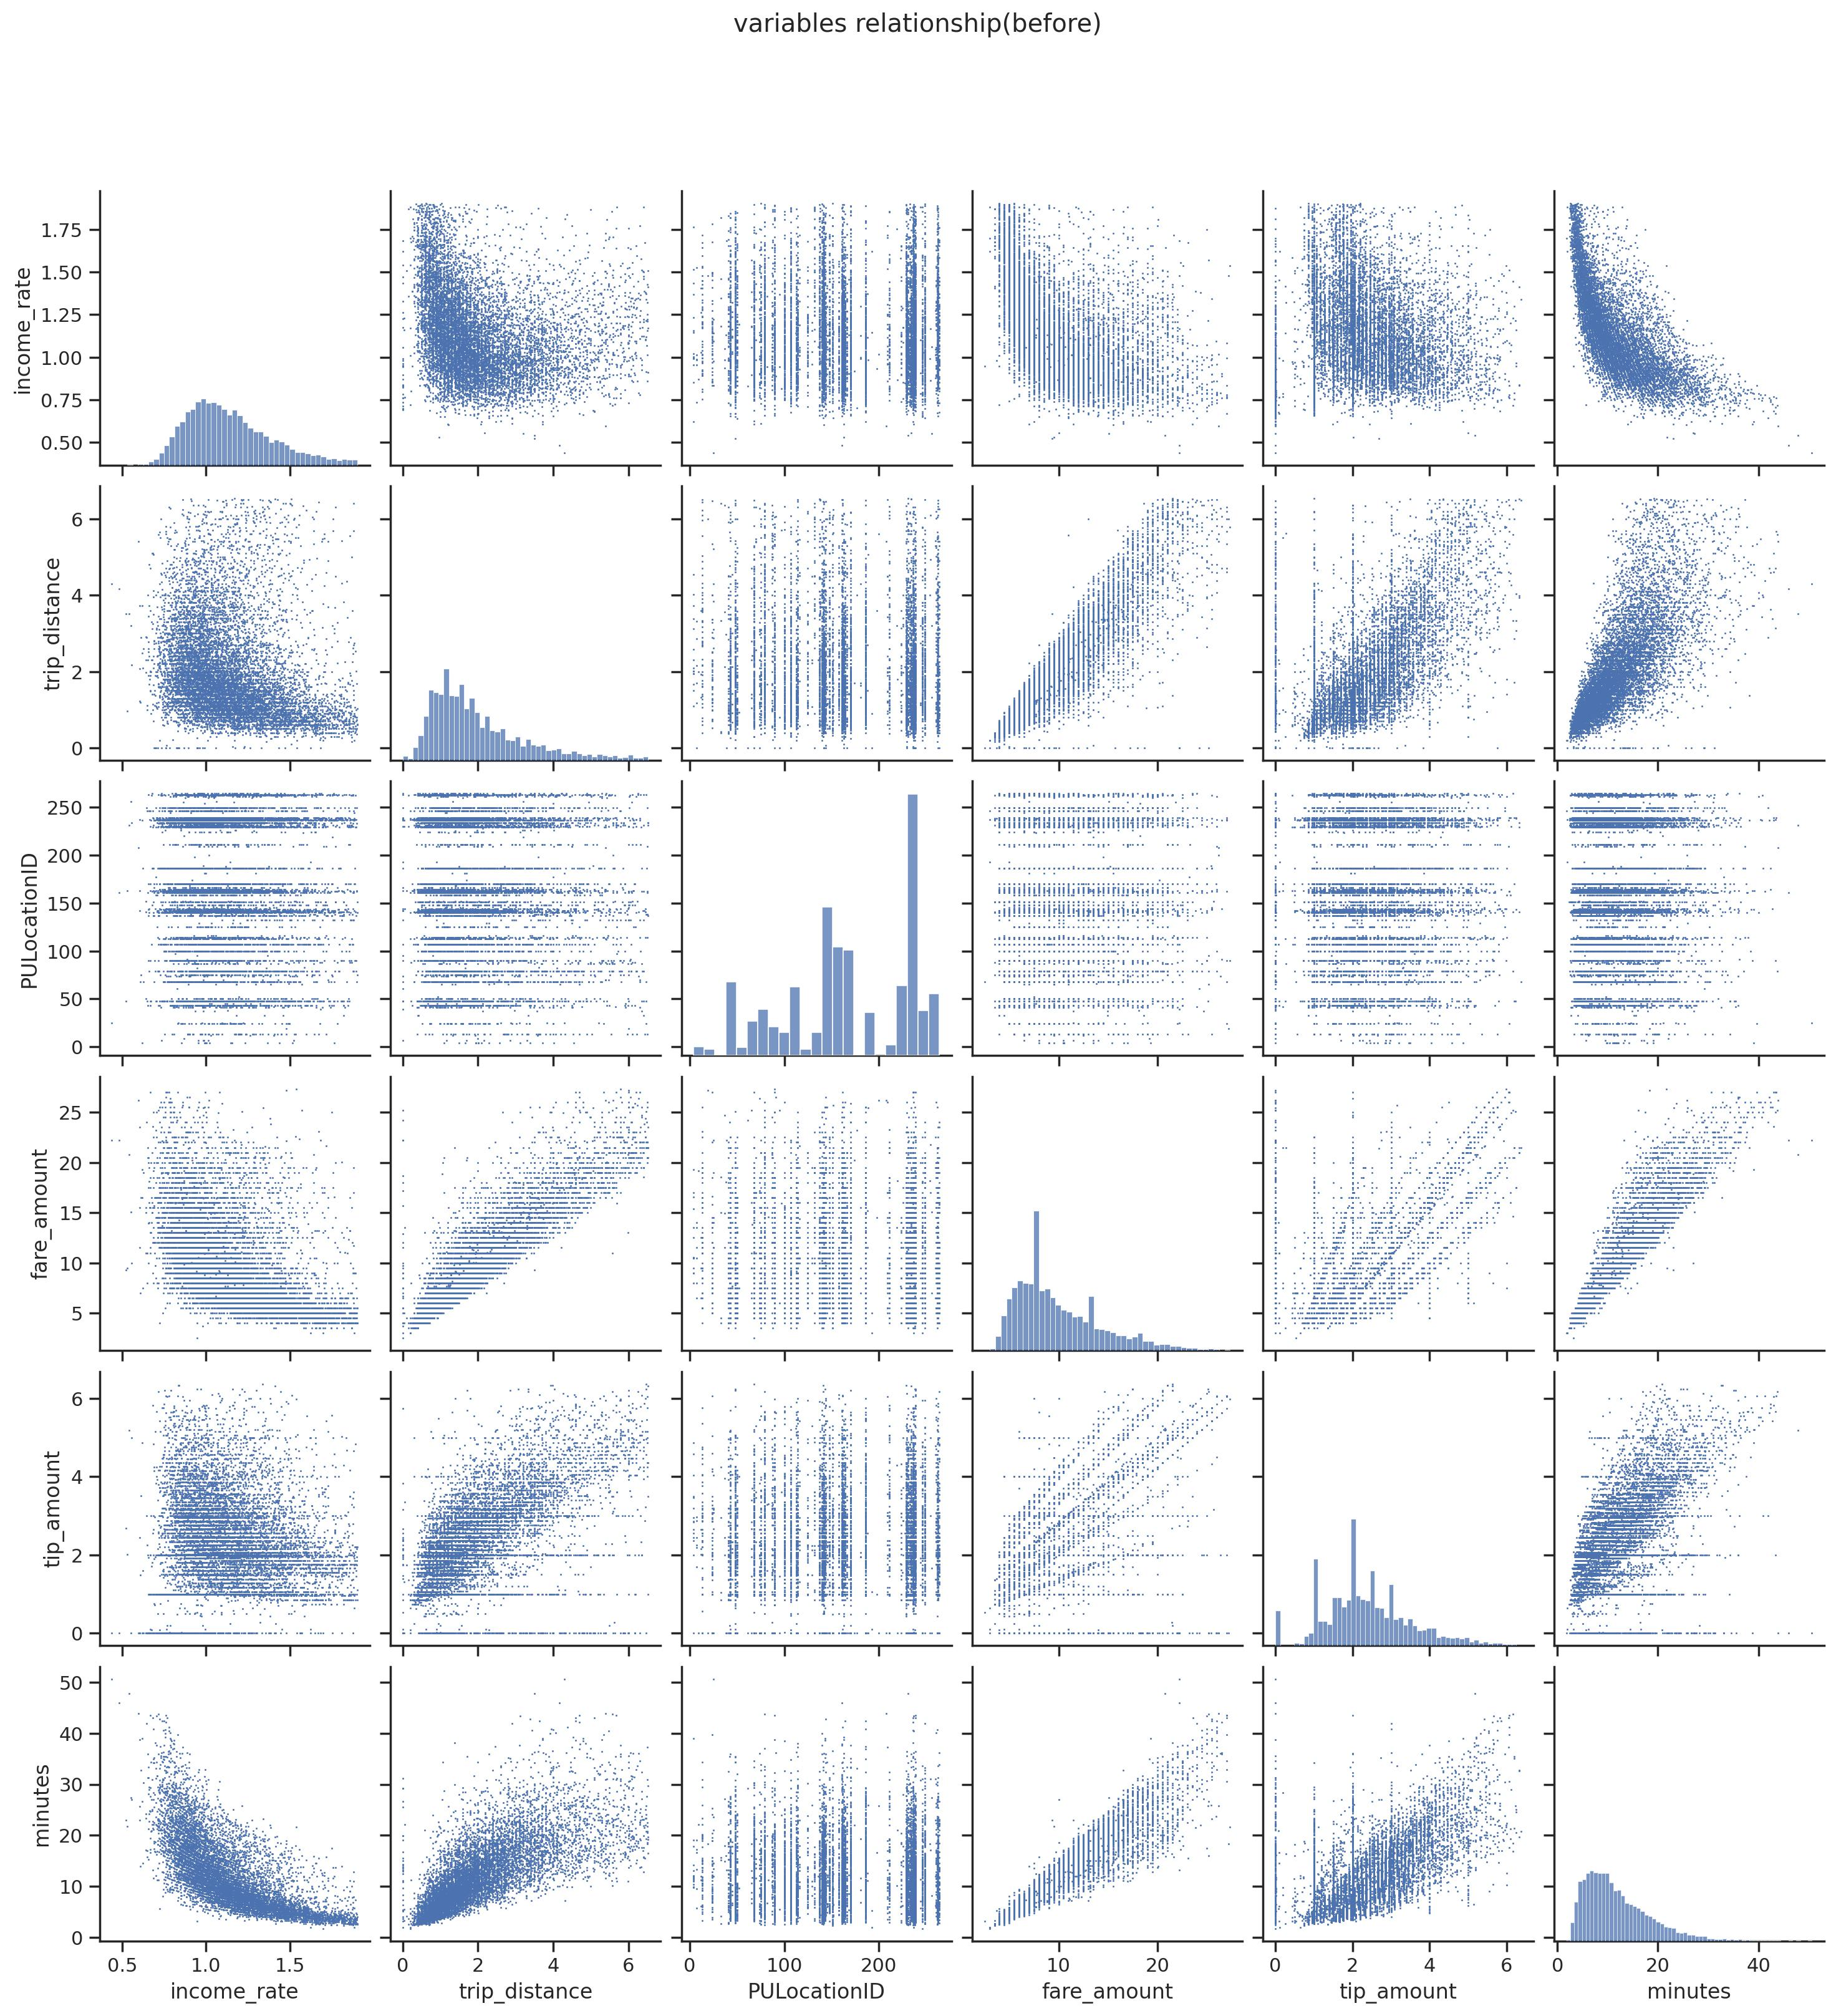
\includegraphics[width=0.9\textwidth]{plots/variables relationship(before).jpg}
  \caption{}
  \label{fig:by:table}
\end{minipage}%
\begin{minipage}{.4\textwidth}
  \centering
  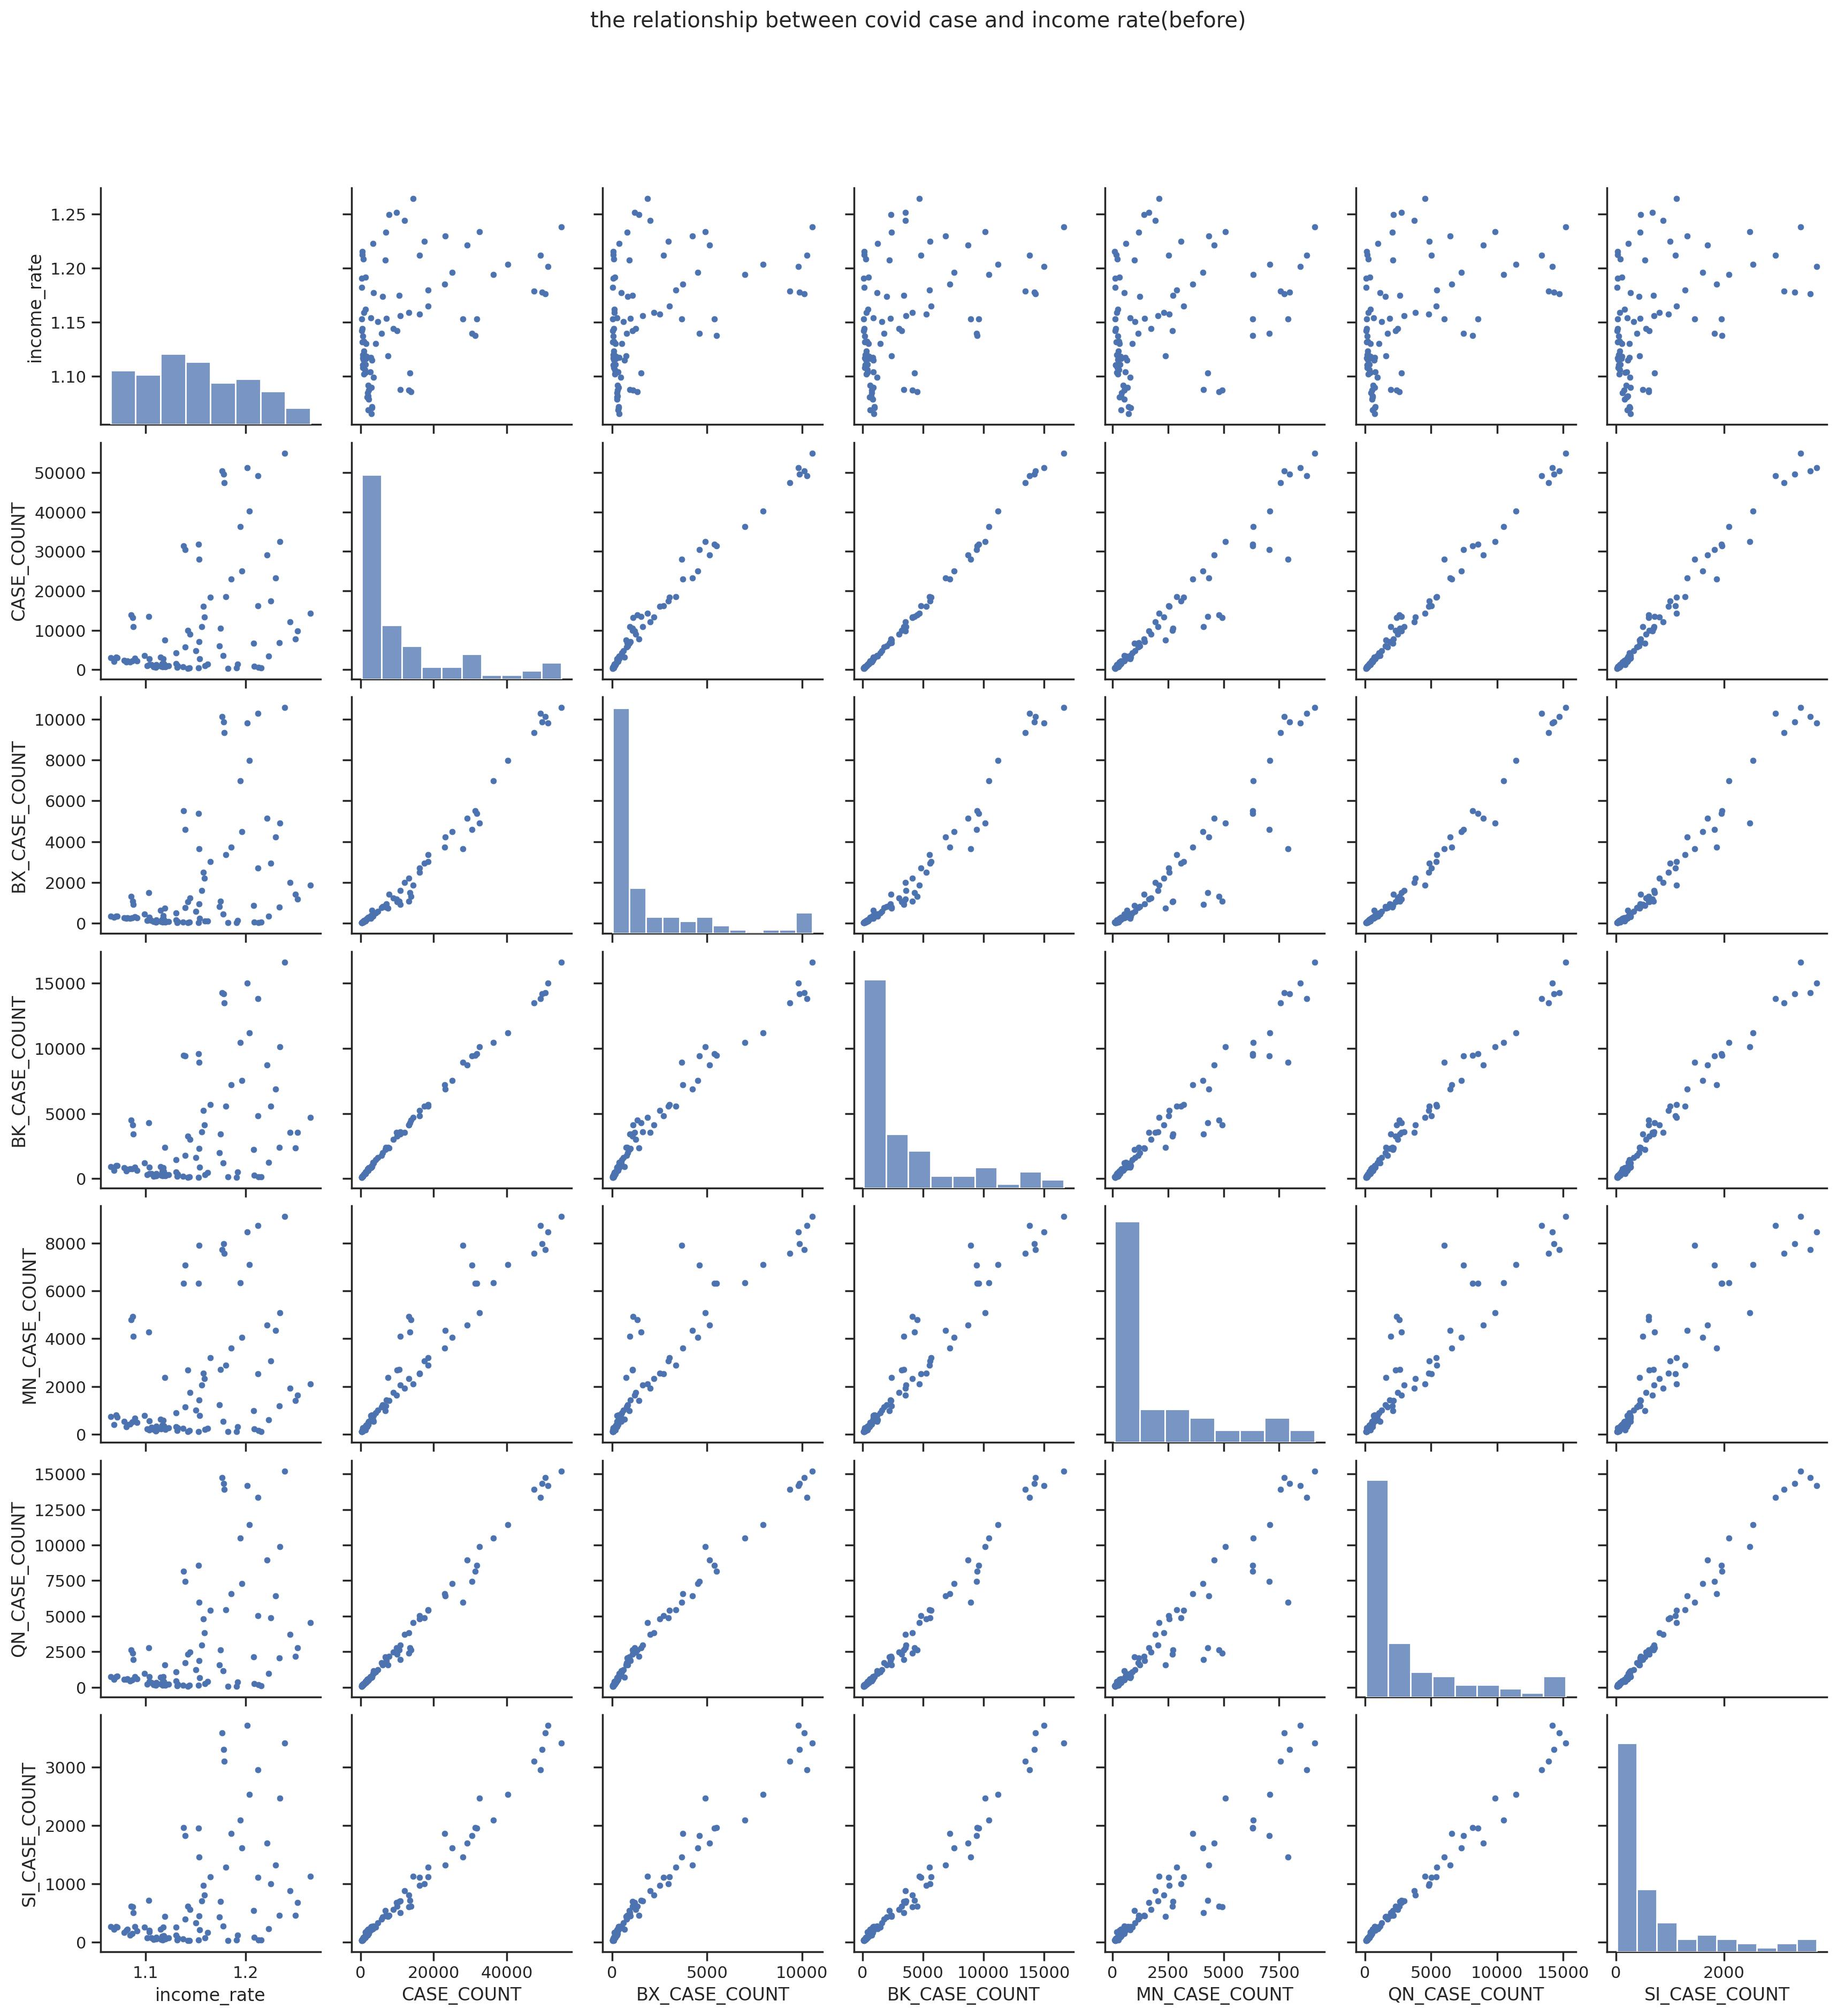
\includegraphics[width=.9\textwidth]{plots/the relationship between covid case and income rate(before).jpg}
  \caption{}
  \label{fig:by:table}
\end{minipage}
\end{figure}
\begin{itemize}
    \item According to Figure 9, it can be seen that after the previous data preprocessing, the variables related to income\_rate are trip\_distance, fare\_amount, tip\_amount, and minutes. These variables basically all increase as income\_rate decreases.
\end{itemize}
\begin{itemize}
    \item According to Figure 10, there is a very strange phenomenon: when the number of COVID-19 increases, the income\_rate of drivers is basically not lower than 1.15. This may be because the New York government has increased the cost of rides for passengers during COVID-19.
\end{itemize}
\section{Map New York}
The upper right corner is the ruler of the income rate of the driver after receiving the order in each area, and the black color means that the driver did not receive the order in that area.
\begin{figure}[H]
    \centering
    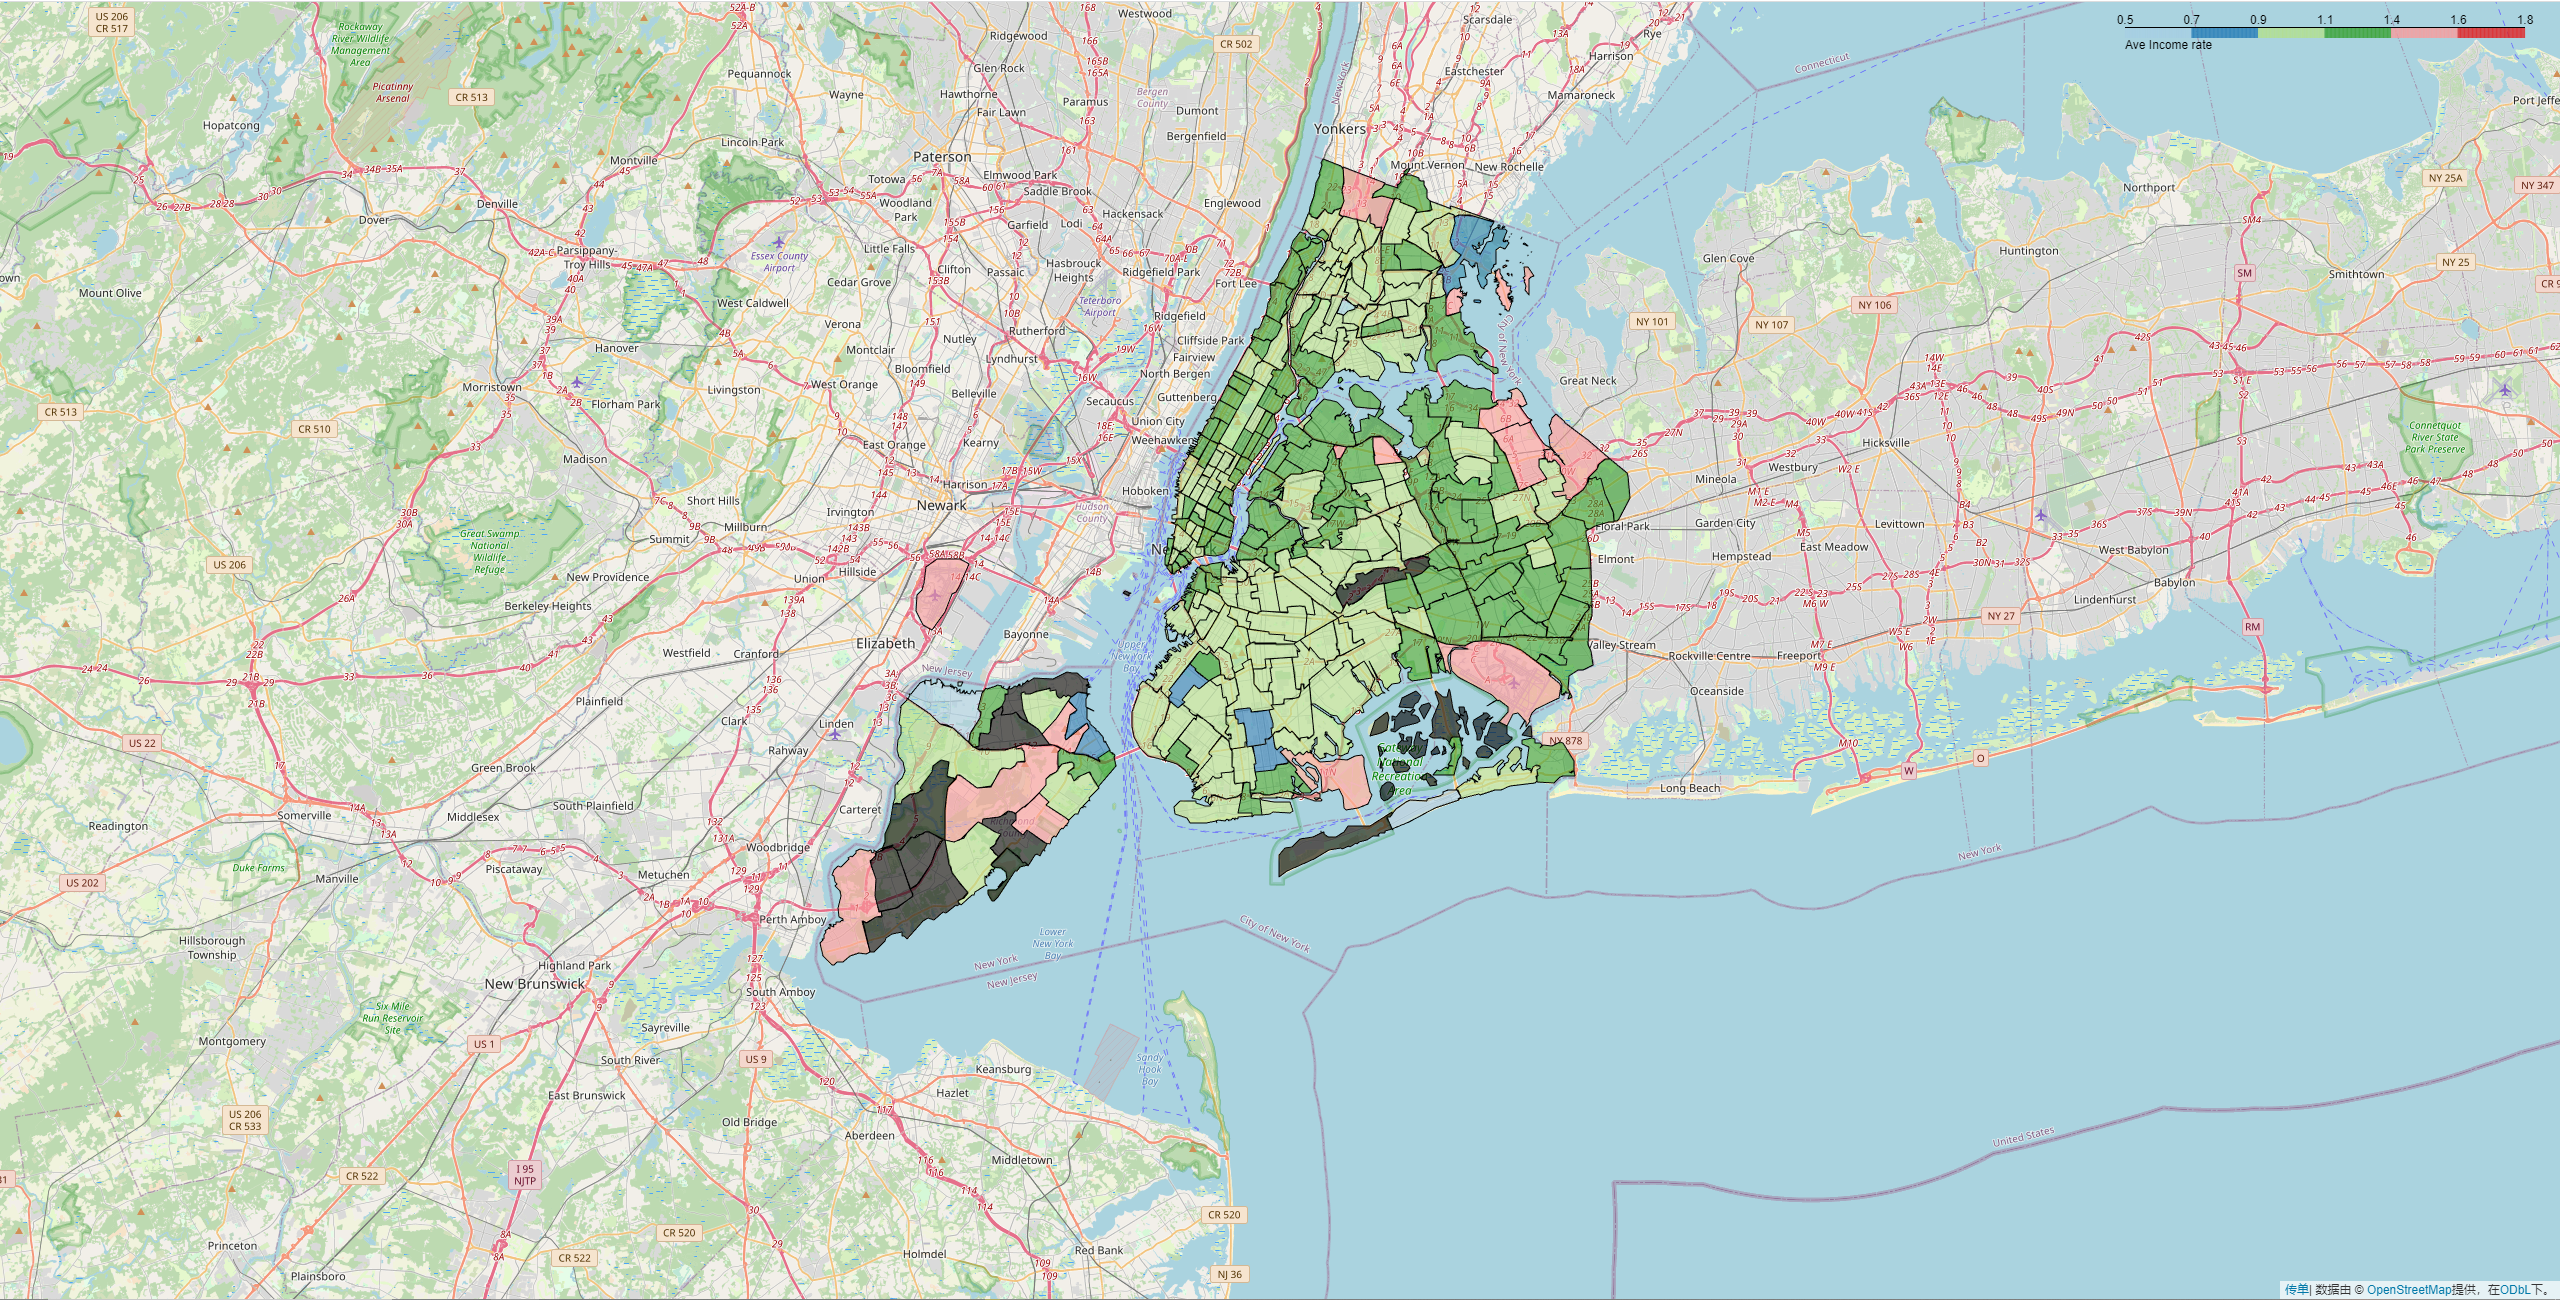
\includegraphics[width=0.8\textwidth]{plots/12-01.PNG}
    \caption{}
    \label{fig:my_label}
\end{figure}
\begin{figure}[H]
    \centering
    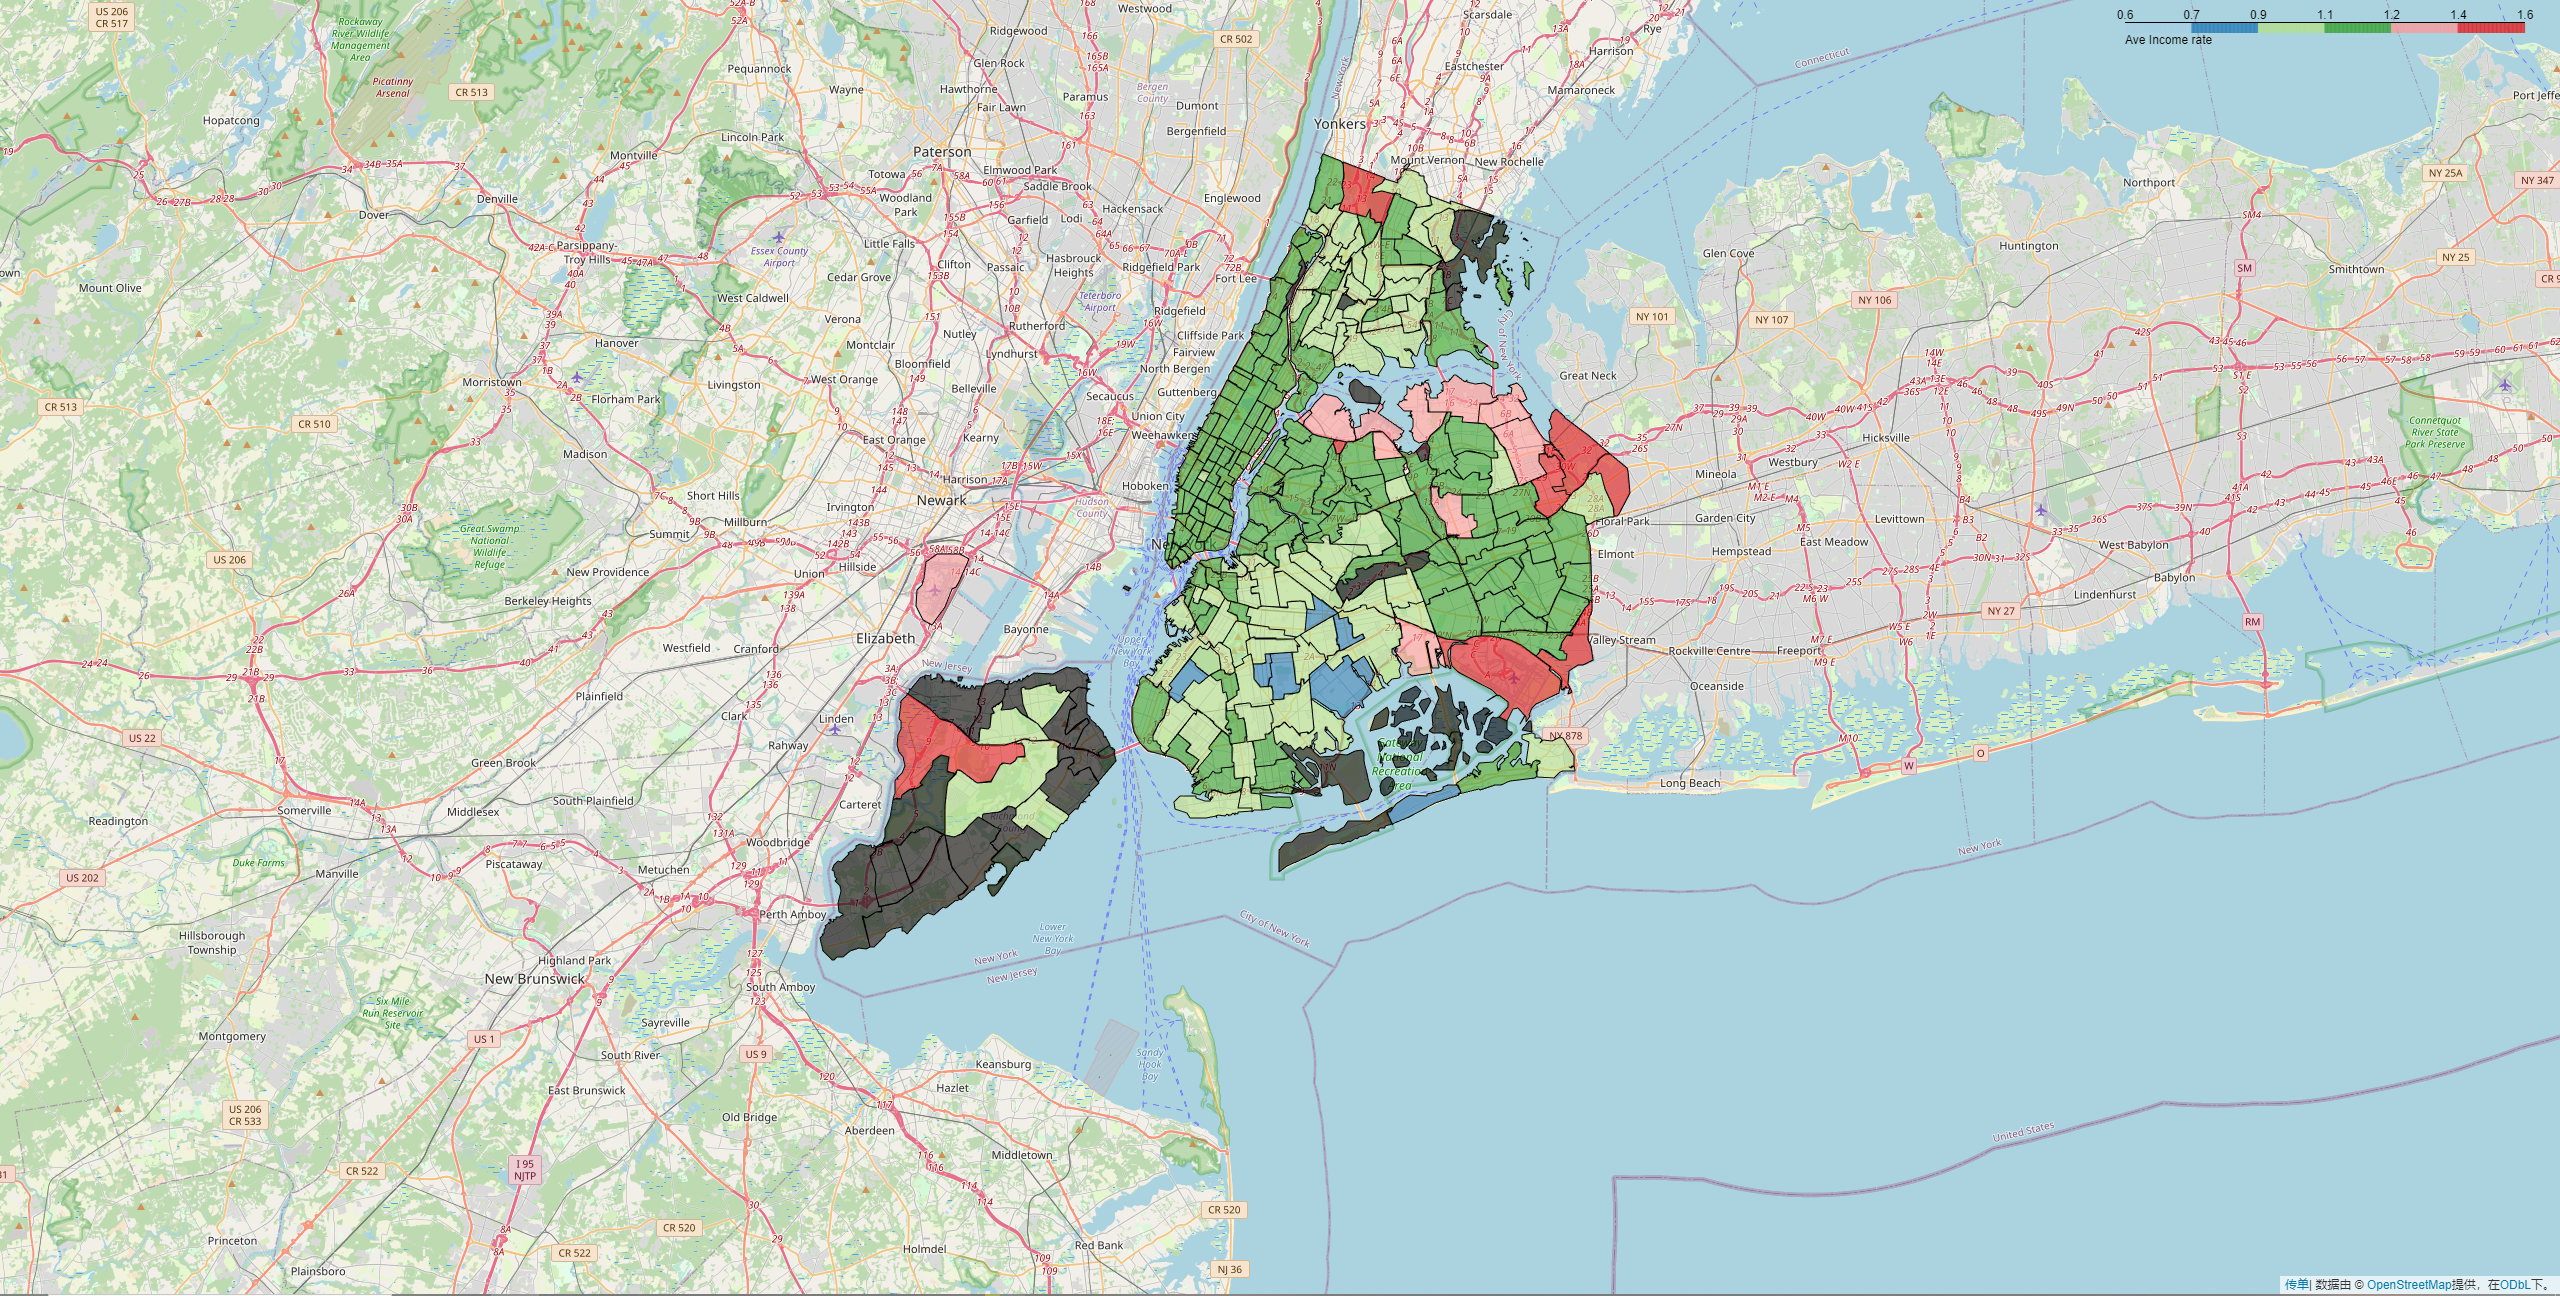
\includegraphics[width=0.8\textwidth]{plots/2.PNG}
    \caption{}
    \label{fig:my_label}
\end{figure}
\begin{figure}[H]
  \begin{minipage}[b]{0.5\textwidth} 
    \centering
    \begin{tabular}{c|c} \hline
    Covid\_period & Count \\
    BX\_CASE\_COUNT &	2603.322581 \\
    BK\_CASE\_COUNT &	4722.516129 \\
    MN\_CASE\_COUNT &	2957.580645 \\
    QN\_CASE\_COUNT &	4281.725806 \\
    SI\_CASE\_COUNT & 1009.096774 \\
    \hline
    \end{tabular} 
    \caption{}
    \label{tab:my_label}
  \end{minipage}% 
  \begin{minipage}[b]{0.5\textwidth} 
    \centering 
    \begin{tabular}{c|c} \hline
    After\_covid & Count \\
    BX\_CASE\_COUNT &	107.250000 \\
    BK\_CASE\_COUNT &	320.785714 \\
    MN\_CASE\_COUNT &	247.964286 \\
    QN\_CASE\_COUNT &	234.428571 \\
    SI\_CASE\_COUNT & 67.321429 \\
    \hline
    \end{tabular} 
    \caption{}
    \label{tab:my_label}
\end{minipage} 
\end{figure}
\begin{itemize}
    \item Figure 11 is the income distribution chart from 12/2021 to 01/2022. During the epidemic, there are large areas on Staten island without orders, and the number of COVID-19 cases on Staten Island is the least (as shown in Figure 13). It is speculated that Staten island may have been closed during the epidemic. A single order in the Queens area with the highest number of outbreaks makes a lot of money, and a few are even pink in the Queens area. Areas that make a lot of money from a single order are generally close to other cities or coastal areas. It is guessed that there are more tourists in these areas, and tourists will give more tips than citizens. However, the Brooklyn area, which also has many epidemics, does not make as much money as a single order in the Manhattan area, which has a moderate number of epidemics. It is difficult to confirm the specific relationship between the number of epidemics and the amount of money earned from a single order.
\end{itemize}
\begin{itemize}
    \item According to Figures 12 and 14, it can be seen that orders in most regions have increased significantly after the number of epidemics has been greatly reduced. But Staten Island has increased black areas, even though it still has the fewest outbreaks in New York City. It is speculated that after the number of epidemics has been greatly reduced, in order to prevent the recurrence of the epidemic, the government has tightened control over Staten Island.
\end{itemize}
\section{Statistical Modelling}
Although according to the chart analysis, it can be seen that the four variables of trip distance, fare\_amount, tip\_amount, and minutes will have an impact on the driver's single order income, and COVID-19 will also affect the income rate. However, in order to have a clearer understanding of the impact of each variable on the income rate and whether it will really affect the income rate, it is necessary to build a model for specific analysis.
This report will choose a linear model to analyze the data(from lecture 3). Linear regression is a statistical analysis method that uses regression analysis in mathematical statistics to determine the quantitative relationship between two or more variables. The reason for choosing it is:
\begin{itemize}
    \item As can be seen from Figure 9 and Figure 10, the number of COVID-19 cases, trip distance, fare\_amount, tip\_amount, and minutes all have a certain linear relationship with income rate, and they are all continuous data.
\end{itemize}
\begin{itemize}
    \item Linear models are simpler and easier to explain to ordinary people.
\end{itemize}
\begin{itemize}
    \item The operation speed of the linear model is very fast. After cleaning the data, there are 7041724 pieces of data left. The time consumption can be minimized by using a linear model.
\end{itemize}
\subsection{yellow taxi data}
\begin{figure}[H]
  \begin{minipage}[b]{0.5\textwidth} 
    \centering
    \begin{tabular}{c|c|c} \hline
    & coef & P\textgreater\left|t\right| \\ \hline    
    intercept & 1.2084 & 0.000 \\
    trip\_distance & -0.0185 & 0.000 \\
    fare\_amount & 0.0662 & 0.000 \\
    tip\_amount & 0.0704 & 0.000 \\
    minutes & -0.0727 & 0.000 \\
    \hline
    \end{tabular} 
    \caption{taxi before trans}
    \label{tab:my_label}
  \end{minipage}% 
  \begin{minipage}[b]{0.5\textwidth} 
    \centering 
    \begin{tabular}{c|c|c} \hline
    & coef & P\textgreater\left|t\right| \\ \hline     
    intercept & 0.0780 & 0.000 \\
    trip\_distance & -0.0093 & 0.000 \\
    fare\_amount & -0.0528 & 0.000 \\
    tip\_amount & -0.0732 & 0.000 \\
    minutes & 0.4702 & 0.000 \\
    \hline
    \end{tabular} 
    \caption{taxi after trans}
    \label{tab:my_label}
\end{minipage} 
\end{figure}
\begin{figure}[H]
  \begin{minipage}[b]{0.5\textwidth} 
    \centering
    \begin{tabular}{c|c|c} \hline
    & coef & P\textgreater\left|t\right| \\ \hline
    Intercept & 1.1333 & 0.000 \\      
    CASE\_COUNT & -0.0053 & 0.004 \\     
    BX\_CASE\_COUNT & 0.0052 & 0.004 \\      
    BK\_CASE\_COUNT & 0.0053 & 0.003 \\     
    MN\_CASE\_COUNT & 0.0052 & 0.004 \\      
    QN\_CASE\_COUNT & 0.0053 & 0.003 \\      
    SI\_CASE\_COUNT & 0.0052 & 0.004 \\     
    \hline
    \end{tabular} 
    \caption{covid before trans}
    \label{tab:my_label}
  \end{minipage}% 
  \begin{minipage}[b]{0.5\textwidth} 
    \centering 
    \begin{tabular}{c|c|c} \hline
    & coef & P\textgreater\left|t\right| \\ \hline
    Intercept & 3.3659 & 0.000 \\      
    CASE\_COUNT & -0.0078 & 0.004 \\     
    BX\_CASE\_COUNT & -0.0077 & 0.004 \\      
    BK\_CASE\_COUNT & 0.0079 & 0.003 \\     
    MN\_CASE\_COUNT & 0.0077 & 0.004 \\      
    QN\_CASE\_COUNT & 0.0078 & 0.003 \\      
    SI\_CASE\_COUNT & 0.0076 & 0.004 \\  
    \hline
    \end{tabular} 
    \caption{covid after trans}
    \label{tab:my_label}
\end{minipage} 
\end{figure}
\begin{figure}
    \centering
    \begin{tabular}{c|c|c} \\ \hline
    & aic & r-squrae \\ \hline
    taxi before trans & -1.100e+04 & 0.698 \\
    taxi after trans & -3.624e+04 & 0.960 \\
    covid before trans & -329.0 & 0.494 \\
    covid after trans & -259.6 & 0.494 \\
    \hline
    \end{tabular}
    \caption{}
    \label{fig:my_label}
\end{figure}
\begin{itemize}
    \item According to Figure 15, it can be concluded that fare\_amount and tip\_amount are positively correlated with income\_rate, and trip\_distance and minutes are negatively correlated with income\_rate. And all four of them have a significant impact on income\_rate. However, since the data shown in Figure 9 is not a complete linear trend but a trend similar to sqrt, and the R-square = 0.698 of the model (R-square represents the degree to which the data is analyzed by the model) is not very high, it is necessary to transform the data. Turn income\_rate into 1/income\_rate, and turn all four variables into sqrt(variables). It can be seen that after the transformation (Figure 19), the AIC of the model has dropped and the R-square has risen to 0.96, which indicates that the data can be basically explained by the linear model, and the results are more accurate. According to Figure 15, it can be seen that the earning efficiency of drivers taking long-distance orders will decrease, and tips will be more important to the earning efficiency of drivers. The reason may be that a driver who takes a long-distance order can only receive a tip from one customer, but at the same time, a driver who takes a short-distance order may have delivered three customers and received three tips.
\end{itemize}
\subsection{COVID-19}
\begin{itemize}
    \item All variables have a significant impact on the income rate. The increase in total cases will reduce the driver's earning efficiency. In addition, the increase in the number of epidemics in each region will increase the driver's earning efficiency. This is strange, it may be that the outbreak of the epidemic caused a large number of drivers to quit, making it difficult for passengers to call a car and had to increase the tip. However, because the growth rate is too slow (the average is only 0.0052), when the number of epidemics increases to a certain extent and the driver's earning efficiency does not increase, it will show a negative correlation. The original images of Covid-19 data and yellow taxi data tend to trend towards sqrt (Figure 10), so transform variables are also needed to make the linear model explain more data. Let income\_rate become sqrt(income). The final result is that the R-square remains unchanged at 0.494 (Figure 19), but the aic drops by 69.4. Later, there was an attempt to use mutual information to test the relationship between total case and income rate, and the result was equal to 4.50, which means that there is a strong connection between the two, indicating that covid data is difficult to fit with a linear model.
\end{itemize}
\section{Recommendation}
\begin{itemize}
    \item It is recommended that drivers work between 3:00 and 6:00. People during this time period may give more tips (figure 7). Drivers better have a rest on Thursdays if they want to relax,  because they are the least efficient in making money on Thursdays (figure 8). It is best to pick up orders in areas that are near to other cities or airports, where drivers are more efficient at making money (Figures 11 and 12).
\end{itemize}
\begin{itemize}
    \item It is best not to take long-distance orders. The longer an order needs to travel, the more time it takes, and the lower the driver's efficiency in making money (figure 15). The current data shows that the epidemic has little effect on drivers’ earning efficiency, so drivers do not need to worry too much about the impact of the epidemic on earning efficiency (figure 17).
\end{itemize}
\vfill
\newpage
\printbibliography





\end{document}